\newcommand{\theory}{

\part{Theory}

\section{Brief Introduction to Semiconductors}

In the world of material science, semiconductors have occupied researchers for centuries and the fascination continues to this day. According to \citet{Busch1989} the word \textit{semiconductor} was first mentioned by Alessandro Volta in 1782 \textit{"...in a paper read in English before the Royal Society in London on 14 March 1782"}.\citep{Busch1989} Later, Michael Faraday would prove the semiconducting properties of materials by showing that increasing temperature could drastically increase the conductivity in certain materials; why this is i will elaborate further on at a later stage.

The photovoltaic (PV) effect, and subsequently photoelectrocemistry, was discovered only a few decades later in 1839 by Edmond Becquerel when he was able to detect a voltage between a solid material and a liquid electrolyte under illumination. \citep{Becquerel1839}

\begin{quotation}
\textit{Dans le dernier Mémoire que j'ai eu l'honneur de présenter à l'Academie, dans sa séance de lundi 29 juliet 1839, je me suis attaché à mettre en évidence, à l'aide des courants électriques, les réactions chimiques qui ont lieu au contact de deux liquides, sous l'influence de la lumière solaire. }
\end{quotation}\vspace*{-.5cm}
\begin{flushright}
\textit{- E. Becquerel, 1839}
\end{flushright}

%With that the foundation for the photovoltaic effect, and subsequently photoelectrocemistry, was laid. What Becquerel showed was that with two Pt

%Already in 1839, A. E. Becquerel reported observation of a voltage between a solid and a liquid electrolyte when struck by light, the photovoltaic effect

%Another important milestone in the history of semiconductors comes with Ferdinand Braun in 1874 when he, at the age of 24, discover the rectification effect at the point of contact between metals and certain crystal materials. This discovery would not find its practical use until the early 1900's when it became an essential part in the development of the radio. This discovery earned Braun the Nobel Prize in physics in 1909. 

\subsection{Understanding the Semiconductor}

The basic idea of semiconductors is easiest explained by showing how atoms and the corresponding electron energies behave when bonding to other atoms, going from single atom electron energies through more complex energy levels in molecules to bands of energy in solids. As shown in figure \ref{fig:energy_bands}, electrons are only allowed to occupy certain energies, or states, and weather these states are filled or not depends on the energy of the electron in question. Instead of 
\begin{figure}[ht!]
\centering
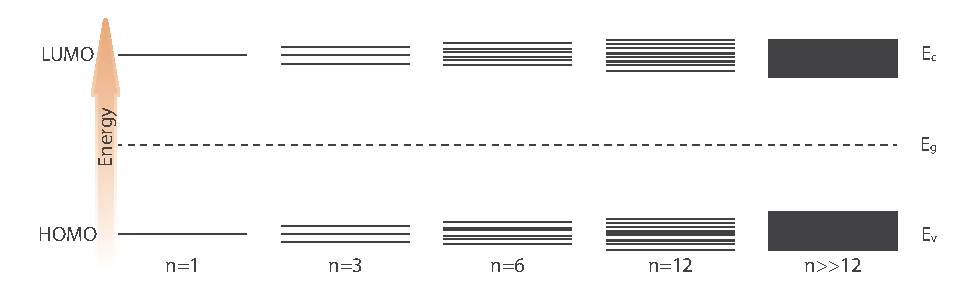
\includegraphics[scale=1]{Figures/Energy_bands1.eps}
\caption{Schematics showing energy bands for different number of atoms}
\label{fig:energy_bands}
\end{figure}

Semiconductors differs from other materials in that the bulk material have certain prohibited electron energy levels. When these atoms come together to form (typically) a crystal, the electron energy levels overlap and from energy levels

%dating back to 18th and 19th when  temperature dependent analysis of the electrical conductivity of Ag$_2$S and Cu$_2$Sn was published in 1851 by Johann Hittorf
%%%%%%%% figure: Parabolic Energy %%%%%%%%%%%%%%%%
	\begin{wrapfigure}{l}{0.5\textwidth}
		\centering
		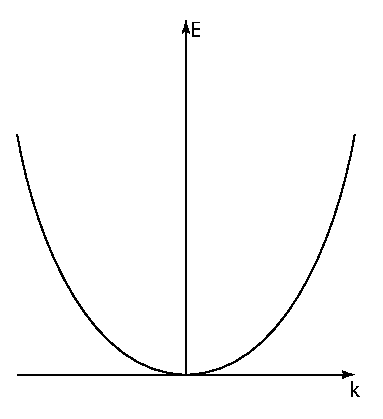
\includegraphics[scale=1]{Figures/Parabolic_energy.eps}
		\caption{Generic Pourbaix diagram for copper}
		\label{fig:pourbaix_generic}
	\end{wrapfigure}
%%%%%%%% end_figure: Parabolic Energy %%%%%%%%%%%%

\section{Electrochemistry}
The current in liquid electrolytes are carried by ions created by dissociation of salts in polar solvents. 

\newpage

\subsection{Pourbaix Diagrams}

Pourbaix diagrams project multiple electrode and electrolyte conditions onto a two dimensional plane and provides information on the corroding conditions as first described by Marcel Pourbaix in his theses dated 1945 \citep{Pourbaix1945}. The two dimensional plot generally depicts three different areas of thermodynamic stability: immunity, passivity and corrosion  as shown in figure \ref{fig:pourbaix_generic}.

%%%%%%%% figure: Pourbaix_generic %%%%%%%%%%%%%%%%
	\begin{wrapfigure}{l}{0.5\textwidth}
		\centering
		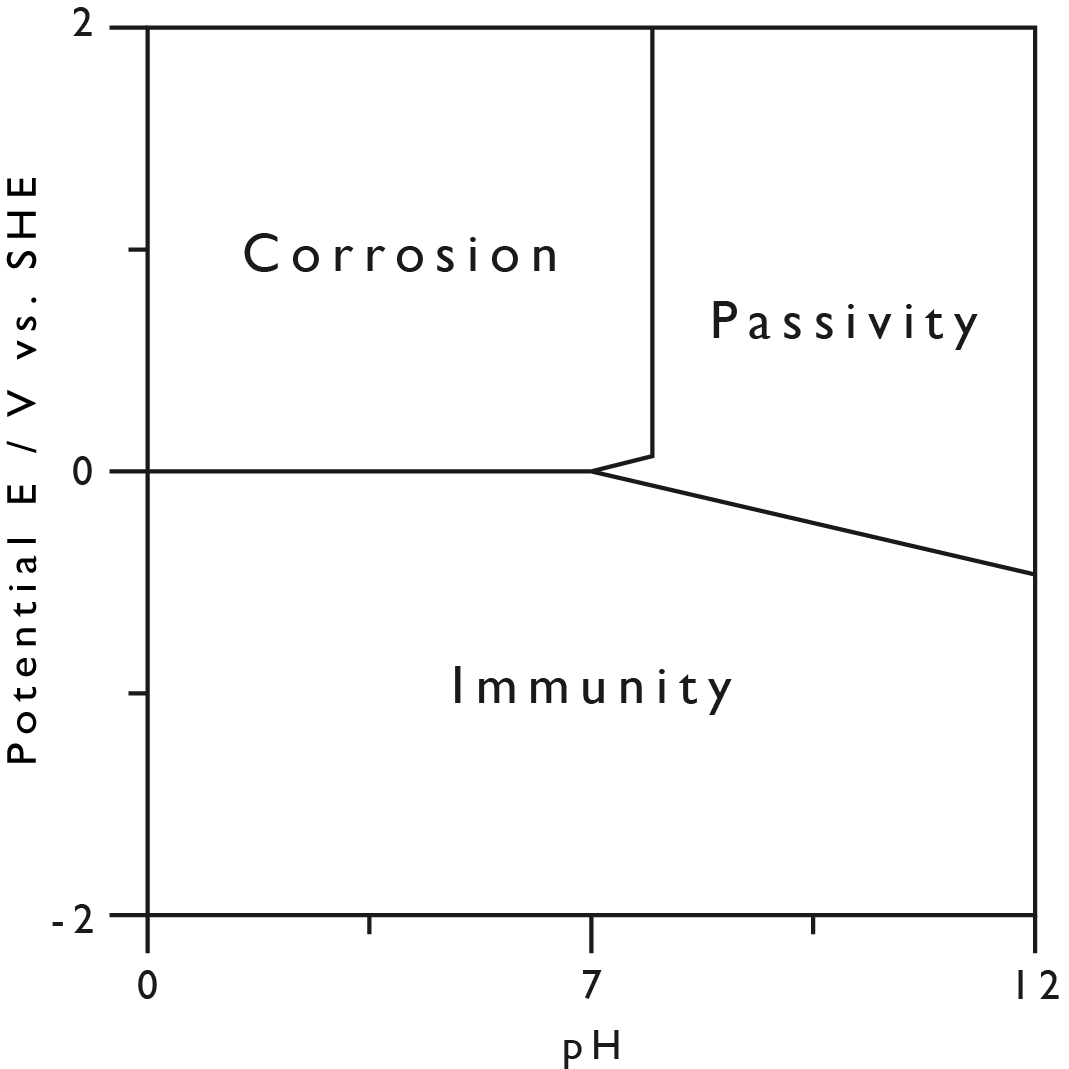
\includegraphics[scale=1]{Figures/pourbaix_generic}
		\caption{Generic Pourbaix diagram for copper}
		\label{fig:pourbaix_generic}
	\end{wrapfigure}
%%%%%%%% end_figure: Pourbaix_generic %%%%%%%%%%%%

The \textit{immunity} zone describes the conditions where the metal itself is the stable phase and corrosion is non-existent. \textit{Passivity} describes the conditions under which the metal is passivated by formation of a coating, usually an oxide or hydroxide. In the corrosion zone, the thermodynamically stable species is a dissolved reaction product, namely metal cations suspended in the aqueous electrolyte \citep{Beverskog1995}.

In a two electrode set-up, one electrode would 

}